\subsection{Osvětlovací modely}
Výpočet osvětlení, záleží na druhu osvětlení a optických vlastnostech těles. Existují 3 základní druhy osvětlení:
\begin{itemize}
 	\item \textbf{Ambientní}  - fiktivní, všudypřítomné, rozptýlené (dopadá na těleso rovnoměrně ze všech směrů).
 	\item \textbf{Difúzní} – matný odraz (intenzita, která se odráží od matného materiálu do všech směrů).
 	\item \textbf{Spekulární}  - odlesk (odrazivá složka – podle zákonů lomu).
\end{itemize}
\subsubsection{Phongův osvětlovací model}
\begin{itemize}
	\item $I = I_a + I_d + I_s$ 
	\item Phongův osvětlovací model je \textbf{empirický} (na fyzice nezaložený) osvětlovací model pro výpočet osvětlení povrchu nějakého objektu.
	\item Ačkoliv tento model není fyzikálně zcela přesný, výsledky, které podává, jsou natolik zdařilé, že se Phongův model v počítačové grafice široce využívá již několik desítek let, zejména pak pro svou rychlost našel uplatnění v real-time grafice.
	\item Jeho \textbf{nevýhodou} je, že nedokáže simulovat některé optické jevy globálního osvětlení, jako např. \textbf{Kaustiky} (Kaustika je obálka světelných paprsků odražených nebo zlomených nějakou zakřivenou plochou nebo předmětem, paprsky na dně bazénu).
		\begin{figure}[H]
		\centering
		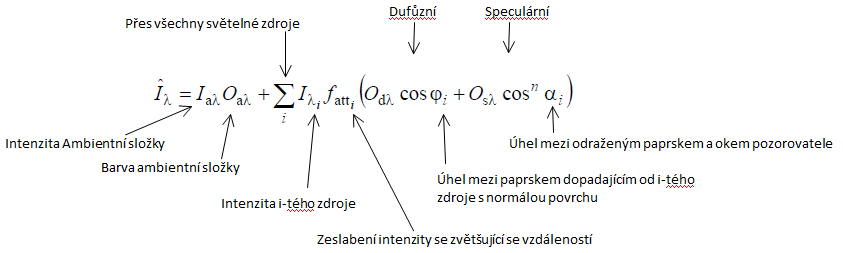
\includegraphics[width=1\textwidth]{assets/1_phong_model}
		\end{figure}
	
\item \textbf{Zeslabení intenzity i--tého světelného zdroje} -- kde $\mathbf{c_0,c_1,c_2}$ jsou konstanty popisující úbytek intenzity světla a $\mathbf{d_i}$ je vzdálenost $f_{att_i} = \min \{\frac{1}{c_0+c_1d_i + c_2d_i^2}, 1\}$.
\item \textbf{Úhel mezi paprskem a normálou} -- kde $n$ je vektor normály plochy, $l_i$ je vektor směřující od místa, kde osvětlení počítám k $i$--tému světelnému zdroji $\cos{\varphi_i} = n \cdot l_i$ (skalární součin).
\begin{figure}[H]
\centering
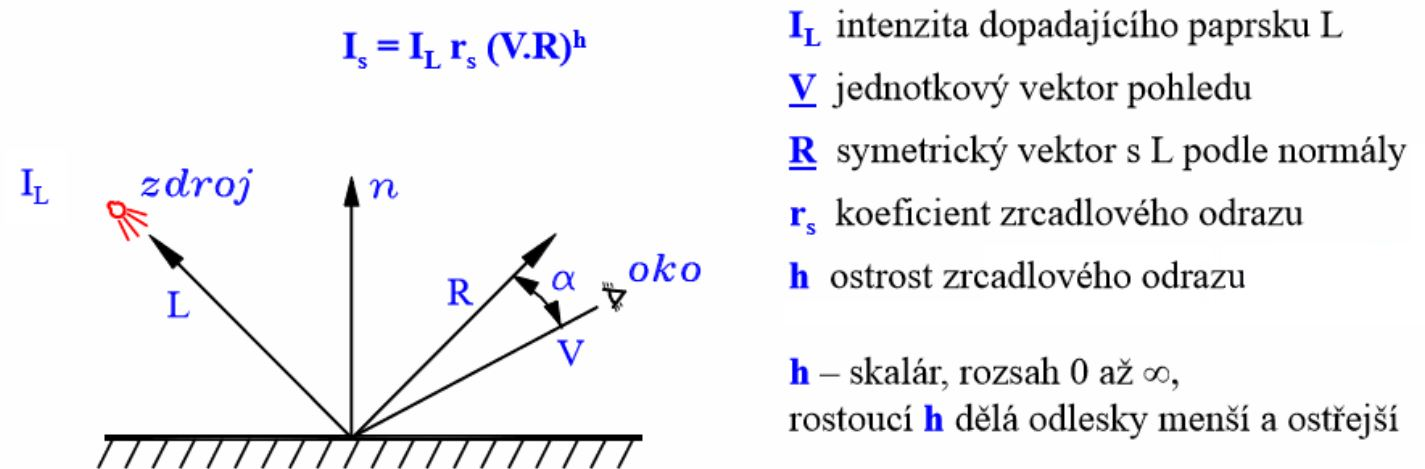
\includegraphics[width=1\textwidth]{assets/1_phong_zrcadlo}
\end{figure}
\end{itemize}

\subsubsection{Blinn-Phong osvětlovací model}
\begin{itemize}
	\item Výchozí osvětlovací model pro standardní zobrazovací řetězec v OpenGL/DirectX. Zavádí tzv. \textbf{half vector}: $ H = \frac{L + V}{| L + V |}$
	\item Místo $R \cdot V$  pak použijeme při výpočtu $N \cdot H$.
	\item Blinn-Phong \textbf{je pomalejší} než původní Phong, protože při výpočtu half vectoru je nutné provést odmocninu (při normalizaci).
	\item Jelikož je odmocnina \textbf{hardwarově implementovaná}, rozdíl je zanedbatelný.
	\item Je však \textbf{rychlejší}, když se pozorovatel a světlo předpokládá v nekonečnu -- směrová světla.
	\item V tom případě je half vector \textbf{nezávislý na poloze a zakřivení povrchu}, stačí jej vypočítat pouze jednou pro každé světlo.
\end{itemize}

\subsection{Systémy barev v PG}
\begin{itemize}
	\item Základem barevného prostoru je \textbf{barevný model}, který nám dává abstraktní matematický popis, jak lze barvy vyjádřit pomocí n-tic čísel, nejčastěji trojic. 
	\item Mezi nejznámější barevné modely v dnešní době patří \textbf{RGB model}. 
	\item Model RGB pracuje se třemi základními barvami: \textbf{červenou, zelenou} a \textbf{modrou}, z nichž se odvíjí i jeho název. 
	\item Tyto barvy byly zvoleny na základně toho, jak \textbf{čípky v lidském oku} vnímají jednotlivé záření. 
	\item Zároveň je RGB \textbf{aditivní barevný model}, což znamená, že se jednotlivé barevné složky \textbf{míchají} (nové barvy získáváme přidáváním větší intenzity jednotlivých složek) a výsledkem jsou další barevné odstíny, případně vyšší intenzita barvy.
	\item Když k tomuto modelu definujeme, jak mají být tyto n-tice interpretovány, dostáváme \textbf{barevný prostor} -- je předem definovaná množina barev, kterou je schopno určité zařízení snímat, zobrazit nebo reprodukovat. 
	\item Barevný prostor je tedy \textbf{definován rozsahem barev}, které dokáže zobrazit. 
	\item Tomuto rozsahu se také říká \textbf{gamut}. Ten se zpravidla zobrazuje jako oblast v CIE 1931 chromatickém diagramu 
\end{itemize}
\begin{figure}[H]
\centering
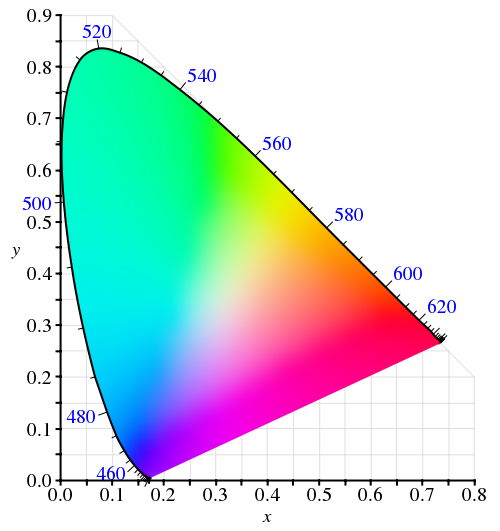
\includegraphics[width=0.3\textwidth]{assets/1_rgb_gamut}
\end{figure}
\subsubsection{RGB}
\begin{itemize}
	\item Nejrozšířenější barevný prostor postavený na RGB barevném modelu je \textbf{sRGB} - standardní RGB. 
	\item Jeho určení je pro zobrazování \textbf{na monitorech} nebo \textbf{kódování barev} na internetu. 
	\item Pro všechny tři barevné složky má definované barvy v \textbf{chromatickém diagramu}, které vymezují jeho gamut. 
	\item Každá barva, kterou tento prostor zobrazuje, je dána zastoupením jednotlivých barevných složek, buďto relativně (hodnoty jsou v rozmezí 0 - 1) nebo absolutně (konkrétní \uv{bitové} hodnoty, zpravidla 0 - 255, 24-bitů).
	\item RGB je možné zobrazit jako krychli.
	\item Často se přidává \textbf{Alpha kanál} pro průhlednost - \textbf{RGBA} (32-bitů).
	\begin{figure}[H]
	\centering
	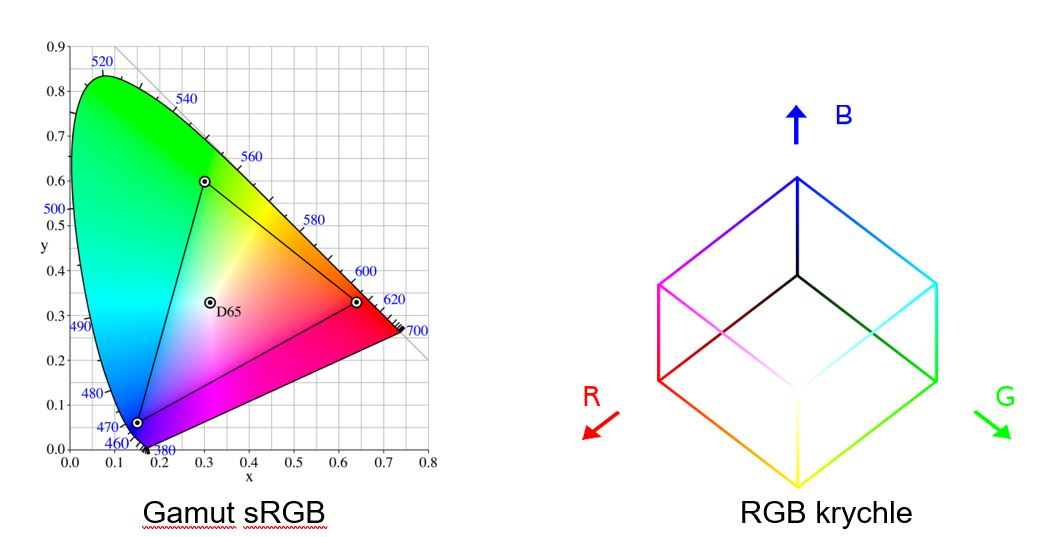
\includegraphics[width=0.6\textwidth]{assets/1_rgb_gamut_krychle}
	\end{figure}
\end{itemize}

\subsubsection{HSV a HSL}
\begin{itemize}
	\item \textbf{Hue, Saturation, Value/Lightness} - barevný model, který nejvíce odpovídá lidskému vnímání barev.
	\item Barvy popisuje pomocí 3 hodnot, které však samy barvy nereprezentují:
	\begin{itemize}
		\item \textbf{Hue} - \textbf{barevný tón}, převládající. Neboli \textbf{odstín} - barva \textbf{odražená} nebo \textbf{procházející} objektem. Měří se jako poloha na standardním barevném kole (\ang{0} až \ang{360}). Obecně se odstín označuje názvem barvy. \ang{0} - červená, \ang{120} - zelená, \ang{240} - modrá.
		\item \textbf{Saturation} - \textbf{sytost} barvy, příměs jiné barvy. Někdy též chroma, síla nebo čistota barvy, představuje množství šedi v poměru k odstínu, měří se v procentech od 0\% (šedá) do 100\% (plně sytá barva). Na barevném kole vzrůstá sytost od středu k okrajům.
		\item \textbf{Value} - \textbf{hodnota jasu}, množství bílého světla. Relativní světlost nebo tmavost barvy. Jas vyjadřuje \textbf{kolik světla barva odráží}, dalo by se také říct přidávání černé do základní barvy.
	\end{itemize}
	\item Nejčastěji se tato reprezentace (popř. \textbf{HSL}) používají v grafických nástrojích jako komponenty pro výběr barvy, protože je mnohem intuitivnější než RGB. 
	\item Vyberu si odstín, jak má být sytý a jasný a hotovo. Není třeba řešit jak smíchat 3 barevné složky, abych dostal to co chci.
	\item Dále se využívá často v případě detekce objektů, kdy hodnota HUE (odstín), je nezávislý na osvětlení scény. Problém však nastává u bílých a černých objektů (kdy HUE může být různé), ty lze na základě value a staturation mapovat do podobných barev (žlutá a černá).
	\item Mimo níže uvedené zobrazení \textbf{válcem}, lze také zobrazit \textbf{kuželem} a 
	\begin{figure}[H]
	\centering
	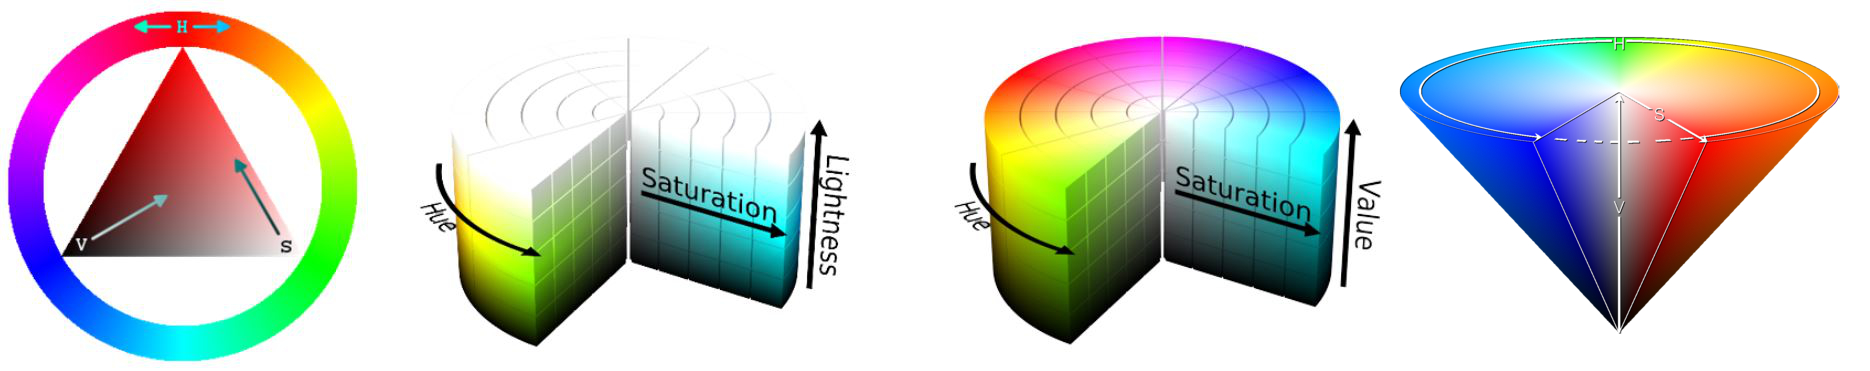
\includegraphics[width=0.9\textwidth]{assets/1_hsv_hsl}
	\end{figure}
\end{itemize}

\subsubsection{CMY a CMYK}
\begin{itemize}
	\item Substraktivní barevné systémy (barvy se ,,\textbf{odečítají}'' od bílé, přidáváním jednotlivých složek až po černou), \textbf{C}yan, \textbf{M}agenta, \textbf{Y}ellow a \textbf{K}ey (Blac\textbf{K}).
	\item Používá se \textbf{pro tisk}.
	\item Černá se přidala, protože smíchání CMY nedává plně černou barvu, navíc je černý inkoust levnější než barevný.
	\item Nevýhodou je, že \textbf{nedokáže správně zobrazit} sytě červenou, zelenou a modrou.
	\item Při tisku to však není poznat.
	\item Před tiskem se RGB obraz převádí do CMYK.
	\item To provádí buďto ovladač tiskárny nebo RIP (Raster Image Processor - u profi tiskáren).
	\item RGB se používá pro aktivní zdroje světla, CMYK jsou \textbf{pasivní} (světlo pouze \textbf{odrážejí}), proto nedokáží udělat tak jasné odstíny.
\end{itemize}
	\begin{figure}[H]
	\centering
	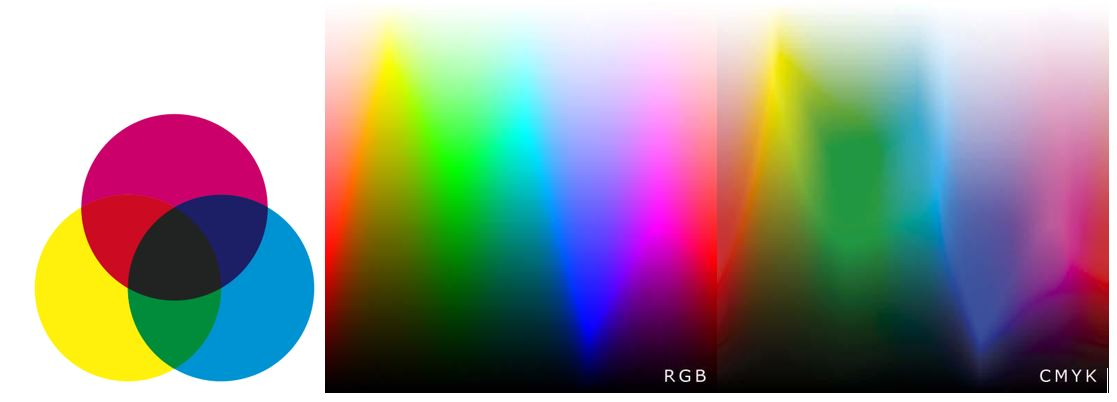
\includegraphics[width=0.6\textwidth]{assets/1_cmyk}
	\end{figure}

\subsubsection{YCbCr}
\begin{itemize}
	\item Barva je reprezentována \textbf{jasovou složkou} Y a modrou a červenou \textbf{chrominanční} komponentou.
	\item Není to absolutní barevný model, jedná se o \textbf{způsob kódování RGB} informací.
	\item Využívá se nejčastěji u videa a barevných obrázků, kde je využito faktu, že \textbf{lidské oko nejvíce vnímá jas}, který je reprezentovaný složkou Y. Barvy už tak důležité nejsou a proto se můžou například více \textbf{komprimovat} bez výraznější ztráty kvality obrazu (JPEG).
	\item Jasová složka je kódována v intervalu $\langle0, 1\rangle$ a chrominanční složky v intervalu $\langle-0.5, 0.5\rangle$
\end{itemize}